\documentclass[12pt]{article}
\usepackage[UTF8]{ctex}
\usepackage{appendix}
\usepackage{enumerate}
\usepackage{amsmath}
\usepackage{graphicx}
\graphicspath{{picture/}}
\usepackage{zhnumber}
\usepackage{cite}
\usepackage{longtable}
\usepackage{array}
\usepackage{bigstrut}
\usepackage{geometry}
\usepackage{multirow}
\usepackage{lastpage}
\usepackage{longtable}
\usepackage{listings}
 \usepackage{color}
  \usepackage{xcolor}
  \lstset{
  language=Matlab,  %代码语言使用的是matlab
  rulesepcolor=\color[RGB]{30,30,30},%代码块边框为淡青色
  backgroundcolor=\color[RGB]{250,250,250},
  keywordstyle=\color[RGB]{0,0,255}\bfseries, %代码关键字的颜色为蓝色,粗体
    numbers=left, % 显示行号
    numberstyle=\tiny,    % 行号字体
   commentstyle=\color[RGB]{0,130,0},    % 设置代码注释的颜色
  showstringspaces=false,%不显示代码字符串中间的空格标记
  stringstyle=\ttfamily, % 代码字符串的特殊格式
  breaklines=true, %对过长的代码自动换行
  extendedchars=false,  %解决代码跨页时,章节标题,页眉等汉字不显示的问题
  escapeinside=``,      % 代码中出现中文必须加上,否则报错
  texcl=true,}
  \lstset{breaklines}
\usepackage[section]{placeins}
\usepackage{mathrsfs}
\usepackage[colorlinks,linkcolor=blue]{hyperref}
\usepackage{titlesec}
\usepackage{titletoc}
\titleformat{\section}{\centering\heiti\zihao{3}}{\zhnum{section}、}{0.3em}{}
\titleformat{\subsection}{\heiti \fontsize{12pt}{0}}{\thesubsection}{0.3em}{}
\usepackage{caption}
\captionsetup[figure]{labelsep=space}
\captionsetup[table]{labelsep=space}
\renewcommand\figurename{\heiti\zihao{5} 图}
\renewcommand\tablename{\heiti\zihao{5} 表}
\renewcommand {\thetable} {\thesection{}.\arabic{table}}
\renewcommand {\thefigure} {\thesection{}.\arabic{figure}}
\renewcommand {\theequation} {\thesection{}.\arabic{equation}}
\date{}
\geometry{a4paper,scale=0.8}

\begin{document}%文档从这里开始。

\numberwithin{footnote}{section}
\renewcommand{\contentsname}{\centering 目录}
\renewcommand{\tablename}{表}
\renewcommand{\figurename}{图}
\renewcommand\refname{参考文献}
\renewcommand\appendix{\setcounter{secnumdepth}{0}}
\renewcommand\abstractname{摘要}
\begin{figure}[h]
  \centering
  \includegraphics[width=.6\textwidth]{logo}
\end{figure}
\thispagestyle{empty}
\begin{center}
\begin{songti}
\zihao{0}\textbf{信号检测与估计}\\
\zihao{1}\ \\\textbf{线性调频脉冲雷达信号处理仿真}\\\ \\\ \\
\zihao{3}
\renewcommand\arraystretch{1.5}
\begin{tabular}{p{1.7cm}<{\centering}p{0.2cm}<{\centering}p{3.6cm}<{\centering}p{1.7cm}<{\centering}p{0.2cm}<{\centering}p{3.5cm}<{\centering}}
作\ \ 者&\textbf{:}&\kaishu{许晓明}&学\  \ 号&\textbf{:}&9161040G0734\\\cline{3-3}\cline{6-6}
学\  \ 院&\textbf{:}&\multicolumn{4}{c}{\kaishu{电光学院}}\\\cline{3-6}
专\ \ 业&\textbf{:}&\multicolumn{4}{c}{\kaishu{电子信息工程}}\\\cline{3-6}
班\ \ 级&\textbf{:}&\multicolumn{4}{c}{\kaishu{电信3班}}\\\cline{3-6}
题 \ \ 目&\textbf{:}&\multicolumn{4}{c}{\kaishu{信号检测与估计}}\\\cline{3-6}
&&\multicolumn{4}{c}{\kaishu{线性调频脉冲雷达信号处理仿真}}\\\cline{3-6}
指导者&\textbf{:}&\multicolumn{4}{c}{\kaishu{顾红}}\\\cline{3-6}
\end{tabular}
\end{songti}
\end{center}
\begin{table}[b]
  \centering
  \zihao{3}
\number\year\ 年\ \number\month月
\end{table}

\begin{center}
\newpage
%\raggedright
\zihao{4}
\newpage
\pagenumbering{Roman}
\setcounter{page}{1}
\tableofcontents
\listoffigures
\newpage
\pagenumbering{arabic}
\end{center}
\section{仿真要求}
\setcounter{page}{1}
\setcounter{table}{0}
\setcounter{figure}{0}
\setcounter{equation}{0}
仿真线性调频脉冲雷达的信号处理。\par设线性调频带宽为34,单位为$MHz$,时宽为$200\mu s$,占空比$10\%$,雷达载频为$10GHz$,输入噪声为高斯白噪声。目标回波输入信噪比可变($-35dB \sim 10dB$),目标速度可变($0 \sim 1000m/s$),目标距离可变($0\sim 10000m$),相干积累总时宽不大于$100ms$。\par 单目标时,给出回波视频表达式;脉压和FFT后的表达式;仿真LFM信号自相关函数,说明第一旁瓣高度,通过内插分析该自相关函数的$4dB$输出脉冲宽度;仿真给出脉压和FFT后的输出图形;通过仿真说明脉压输出和FFT输出的SNR;仿真说明脉压时多卜勒敏感现象和多卜勒容限及其性能损失(脉压主旁比与多卜勒的曲线);仿真说明距离模糊和速度模糊的情况。\par 双目标时,仿真出大目标旁瓣(距离和速度旁瓣)盖掩盖小目标的情况;仿真出距离分辨和速度分辨的情况。
\section{线性调频信号(LFM)原理}
\setcounter{table}{0}
\setcounter{figure}{0}
\setcounter{equation}{0}
\subsection{线性调频脉冲雷达}
雷达发射机产生雷达波形,然后经馈线和收发开关由发射天线辐射出去,遇到目标后,电磁波一部分反射,经接收天线和收发开关由接收机接收,对雷达回波信号做适当的处理就可以获知目标的相关信息。\par
当目标与雷达的相对距离为$R$,为了探测这个目标,雷达发射信号$s(t)$,电磁波以光速$C$向四周传播,经过时间$R/C$后电磁波到达目标,照射到目标上的电磁波可写成:$s(t-\frac{R}{C})$。电磁波与目标相互作用,一部分电磁波被目标散射,被反射的电磁波可记为
$\sigma s(t-\frac{R}{C})$,其中$\sigma$为目标的雷达散射截面(RCS),反映目标对电磁波的散射能力,(在仿真中,我以目标幅度$A$代替$\sigma$进行仿真,即反射电磁波为$A s(t-\frac{R}{C})$)再经过时间$R/C$后,被雷达接收天线接收的信号为$A s(t-\frac{2R}{C})$。\par
脉冲压缩雷达可以同时提高雷达的作用距离和距离分辨率。这种雷达采用宽脉冲发射以提高发射的平均功率,因而有足够大的作用距离;而在接收时采用脉冲压缩算法获得窄脉冲,以提高距离分辨率,较好的解决雷达作用距离与距离分辨率之间的矛盾。\par
脉冲压缩雷达最常见的调制信号是线性调频(LFM)信号,接收时采用匹配滤波器压缩脉冲。
\subsection{线性调频信号(LFM)}
LFM信号的数学表达式为:
\begin{equation}\label{LFM1}
  s(t)=\mbox{rect}(\frac{t}{\tau})e^{j2\pi\left(f_ct+\frac{K}{2}t^2\right)}
\end{equation}
其中,$K=\frac{B}{\tau}$为调频斜率,$\mbox{rect}(\frac{t}{\tau})$为矩形信号,满足
\begin{equation}\label{juxing1}
\mbox{rect}(\frac{t}{\tau})=\left\{
  \begin{array}{ccc}
    1 &,&\vert \frac{t}{\tau}\vert \leq 1 \\
    0 &,& \mbox{其他} \\
  \end{array}
  \right.
\end{equation}
LFM信号又可表示为
\begin{equation}\label{wuzaipinLFM}
\begin{array}{c}
  s(t)=s'(t)e^{j2\pi f_ct}\\
  s'(t)=\mbox{rect}(\frac{t}{\tau})e^{j\pi Kt^2}
\end{array}
\end{equation}
$s'(t),s(t)$在傅里叶变换后具有相同的幅频特性,仅仅是载频不同,信号仿真时,可以用$s'(t)$进行模拟。\par
\section{单目标时的仿真情况}
\setcounter{table}{0}
\setcounter{figure}{0}
\setcounter{equation}{0}
\subsection{LFM信号}
利用补零的方式,产生线性调频脉冲信号,其波形见图\ref{LFM2}
。
\begin{figure}[htbp]
  \centering
  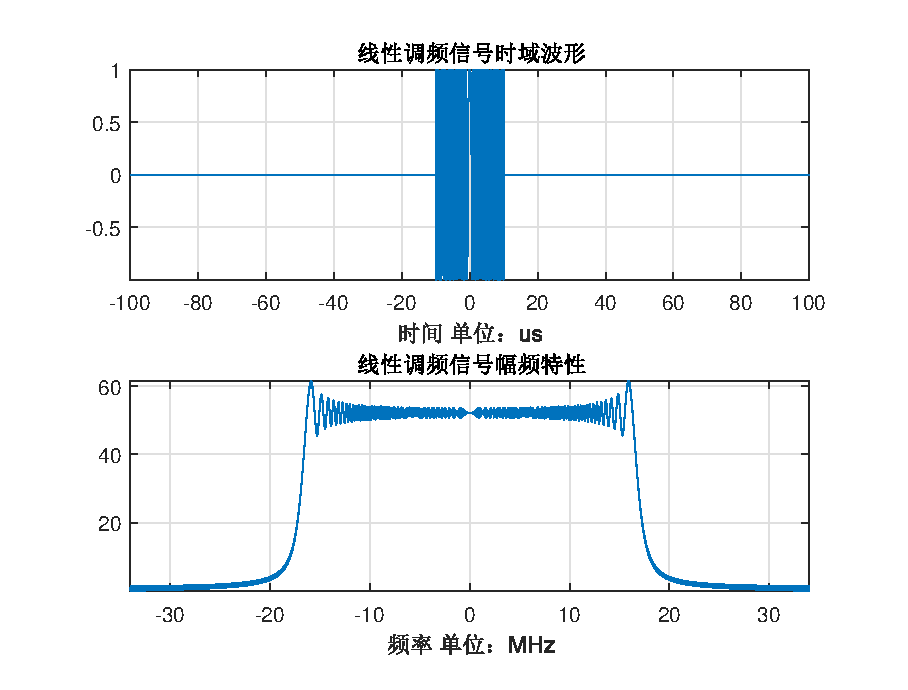
\includegraphics[width=\textwidth]{fasheboxing}
  \caption{LFM信号波形情况}\label{LFM2}
\end{figure}
\subsection{自相关函数}
\subsubsection{自相关函数表达式及图像}
在信号处理中,自相关函数的定义为
\begin{equation}\label{zixiangguanhanshu}
  r(t)=\int_{-\infty}^{+\infty}s(t+\tau)s^*(\tau)\mbox{d}\tau=s(t)*s^*(-t)
\end{equation}
因此LFM信号的自相关函数可通过卷积定理转换到频域处理
\begin{equation}\label{zixiangguanhanshu2}
\left\{
\begin{array}{c}
   R(\omega)=S(\omega)\cdot S^*(\omega) \\
  r(t)=\mathscr{F}^{-1}[R(\omega)]\\
\end{array}
\right.
\end{equation}
同时,直接计算\ref{zixiangguanhanshu},又可得
\begin{equation}\label{zhijiejisuan}
r(t)=\left\{
  \begin{array}{ccc}
   \frac{\sin(\pi K (\tau-t)t)}{\pi K t}e^{j2\pi f_c t} &,& 0 \leq t\leq \tau\\
    \frac{\sin(\pi K (\tau+t)t)}{\pi K t}e^{j2\pi f_c t} &,& -\tau \leq t\leq 0 \\
  \end{array}
  \right.
\end{equation}
整理,得
\begin{equation}\label{zixiangguanhanshuyupipeilvboxiang}
r(t)=\tau\frac{\sin(\pi K (\tau-|t|)t)}{\pi K t\tau}e^{j2\pi f_c t}\mbox{rect}(\frac{t}{2\tau})
\end{equation}
于是,自相关函数波形见图\ref{zxghs}
。
\begin{figure}[htbp]
  \centering
  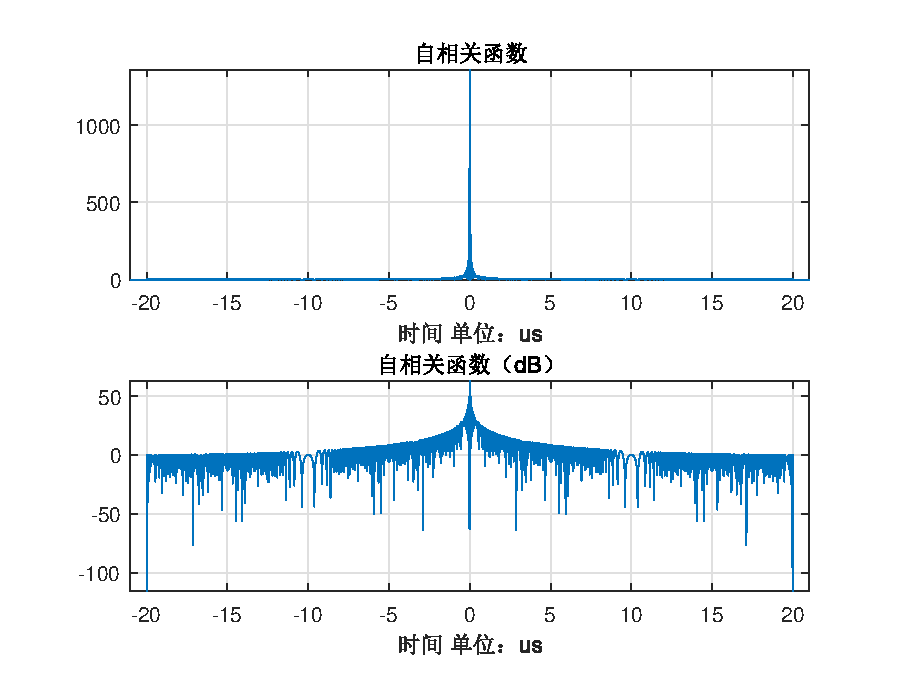
\includegraphics[width=\textwidth]{zxghs}
  \caption{自相关函数波形}\label{zxghs}
\end{figure}
\subsubsection{自相关函数相关参数}
\par查看仿真图数据,为了更好地找到4dB输出脉冲宽度,对自相关函数进行归一化处理,数据见图\ref{zxghs2}
。
\begin{figure}[htbp]
  \centering
  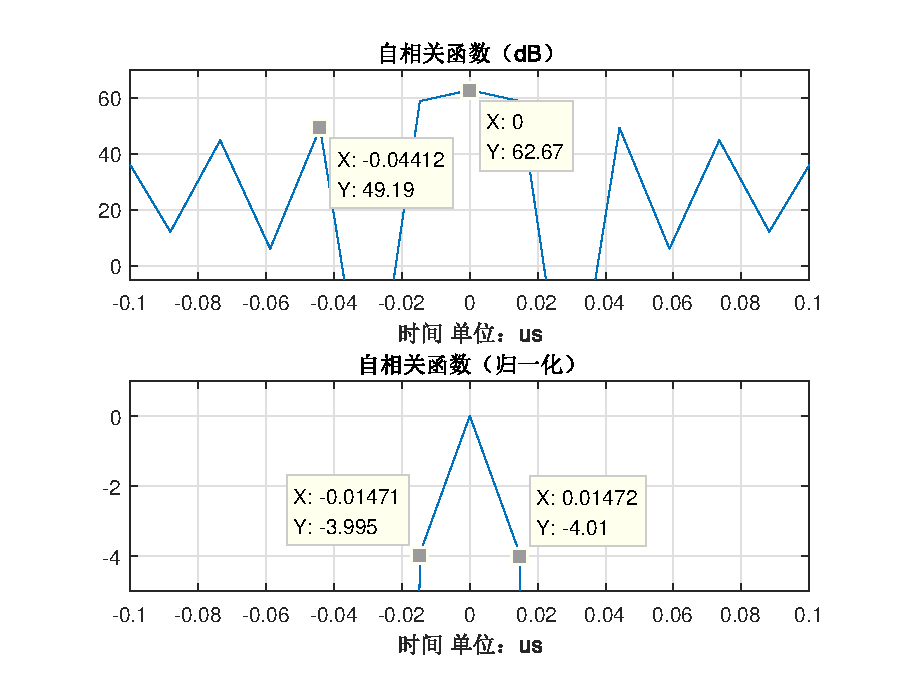
\includegraphics[width=\textwidth]{zxghsshuju}
  \caption{自相关函数相关参数-由图像所得}\label{zxghs2}
\end{figure}
\par由图中数据,得到表\ref{1111}
\begin{table}[h]
  \centering
  \caption{}
\begin{tabular}{|c|c|}
  \hline
    主瓣高度&62.67dB\\\hline
    旁瓣高度&49.19dB\\\hline
    主旁瓣比&13.48dB\\\hline
    4dB输出脉宽&0.02943$\mu s$=29.43$ns$\\\hline
  \end{tabular}
  \label{1111}
\end{table}
\par编写matlab代码查找对应位置,数据见图\ref{zxghs3}
,表\ref{1222}
\begin{table}[htbp]
  \centering
  \caption{ }
  \begin{tabular}{|c|c|}
    \hline
    主瓣高度&62.6708dB\\\hline
    旁瓣高度&49.1931dB\\\hline
    主旁瓣比&13.4776dB\\\hline
    4dB输出脉宽&29.4139$ns$\\
    \hline
  \end{tabular}
  \label{1222}
\end{table}
\begin{figure}[htbp]
  \centering
  \includegraphics[width=.6\textwidth]{TIM20190602205603}
  \caption{自相关函数相关参数-MATLAB编码求得}\label{zxghs3}
\end{figure}
\subsubsection{误差情况分析}
由式(\ref{zixiangguanhanshuyupipeilvboxiang}),当$|t|$远远小于$\tau$时,可认为
\begin{equation}\label{yuanxiaoyushi}
  r(t)\approx\tau\mbox{Sa}(\pi K\tau t)\mbox{rect}(\frac{t}{2\tau})
\end{equation}
对于辛格函数而言,其主瓣下降4dB对应的宽度与第一零点值大致相等,而式(\ref{yuanxiaoyushi})的第一零点为$t=\frac{1}{K\tau}=\frac{1}{\frac{B}{\tau}\tau}=29.4118ns$。仿真得到的实际值与理论值相对误差为0.0071\%
\subsection{回波信号}
回波信号表达式为:
\begin{equation}\label{huiboxinhaao}
  \begin{array}{rl}
  s_r(t)&=A\mbox{rect}(\frac{t}{T})e^{j2\pi\left(\left(f_c+f_d\right)\left(t-t_r\right)+K\left(t-t_r\right)^2\right)}   \\
  & =As(t-t_r)e^{j2\pi f_d\left(t-t_r\right)}\\
  \end{array}
\end{equation}
其中,$t_r$为回波目标延时,$t_r=\frac{2R}{C}$;$f_d$为多普勒频移,$f_d=\frac{2v}{\lambda}$。
回波信号波形示意图见图\ref{huiboboxingtu}
。
\begin{figure}[htbp]
  \centering
  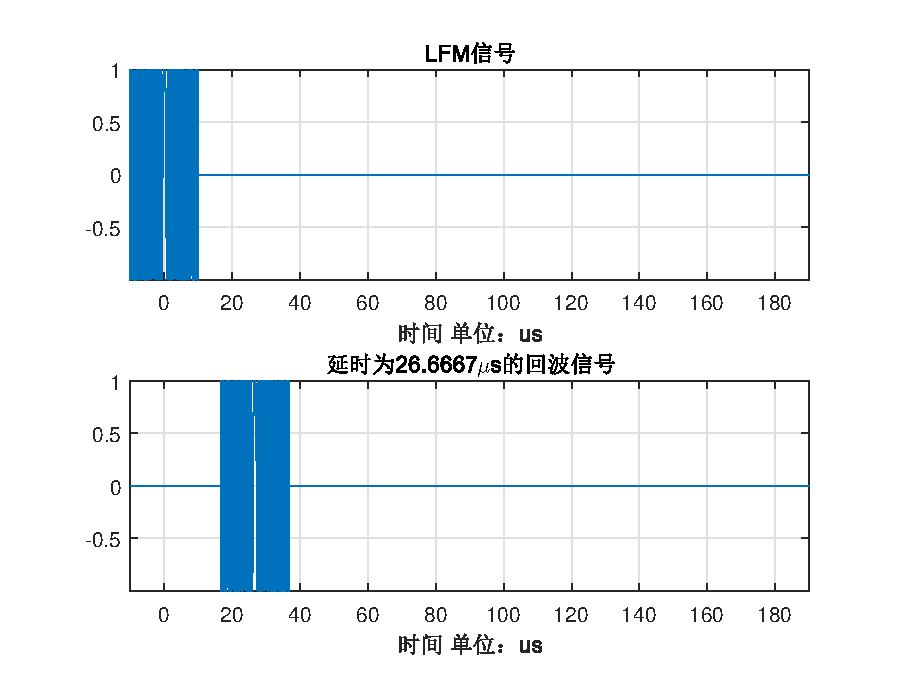
\includegraphics[width=\textwidth]{huiboxinghao}
  \caption{回波波形示意图}\label{huiboboxingtu}
\end{figure}
\subsection{脉冲压缩(匹配滤波)}
\subsubsection{脉冲压缩表达式及图像}
在白噪声背景下,所得输出信噪比最大的线性滤波器就是匹配滤波器,其冲击响应满足为
\begin{equation}\label{chongjixiangying}
  h(t)=ks^*(T-t)
\end{equation}\par
k为滤波器的相对放大量,可以取k=1。于是匹配滤波后的回波表达式为
\begin{equation}\label{pipeilubohou}
  s_h(t)=h(t)*s_r(t)=s_r^*(T-t)*s_r(t)
\end{equation}
与自相关函数的情况大致相同,则其表达式可参见式(\ref{zixiangguanhanshuyupipeilvboxiang})。\par
加入噪声后,脉冲压缩前后的图像见图\ref{maichongyasuotuxiang}
。
\begin{figure}[htbp]
  \centering
  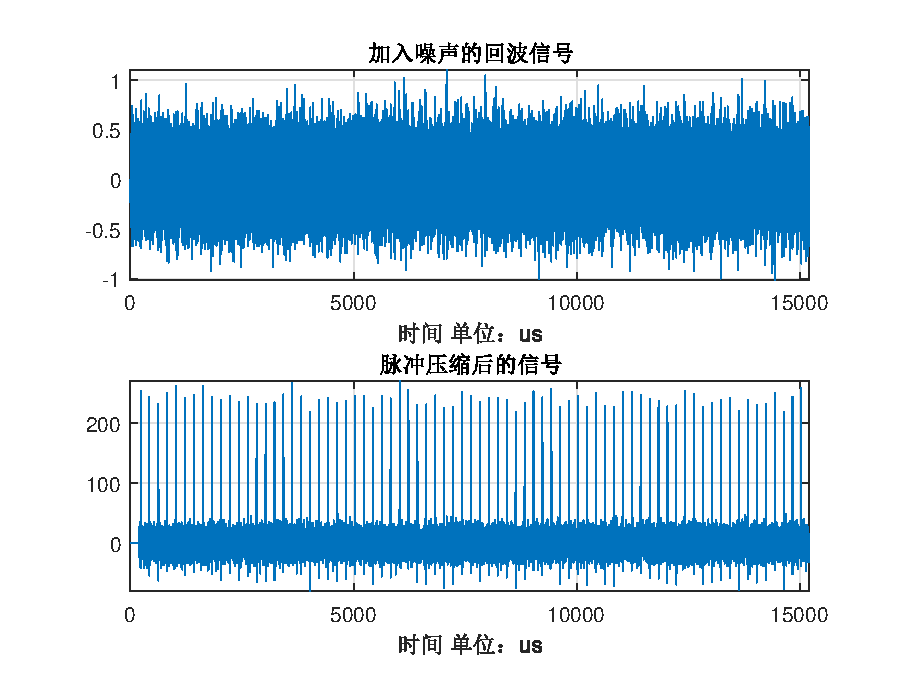
\includegraphics[width=\textwidth]{maiyaqianhou}
  \caption{脉冲压缩前后图像}\label{maichongyasuotuxiang}
\end{figure}
\subsubsection{脉压输出SNR及误差情况分析}
由于噪声带宽与信号带宽不一致,故通过低通滤波器调节,使得二者功率谱带宽大致相等,参见图\ref{tiaojiezhong}
。从图中可以看到,通过低通滤波器后的噪声功率谱带宽与信号带宽大致相等。\par
对于LFM信号而言,脉冲压缩前的时宽$\tau=T/10$,脉冲压缩后,由\ref{zixiangguanhanshuyupipeilvboxiang},可知当$|t|$远远小于$\tau$时,4dB时宽为$1/B$,于是,脉冲压缩增益理论值为
\begin{equation}\label{zengyi1}
 D_{theory}=\frac{\tau}{\frac{1}{B}}=B\tau=680=28.3251\mbox{dB}
\end{equation}
当输入信噪比$SNR_i$设定为-5dBs时,理论输出信噪比${SNR_o}_{thero}=23.3251$dB。由图\ref{shuju_pipeilvbo}
可知,其实际输出信噪比$SNR_o=23.4692$dB,相对误差为$0.6178\%$。产生误差的原因可能是低通滤波器不能做到恰好滤去所有高频分量,以及信号、噪声功率谱带宽不完全相等。
\begin{figure}[htbp]
  \centering
  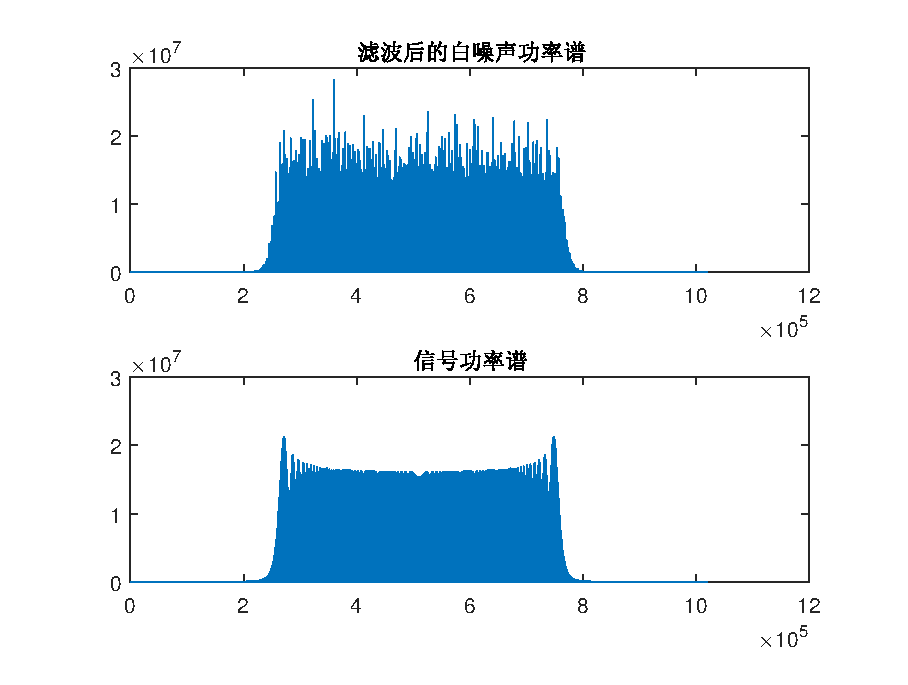
\includegraphics[width=\textwidth]{tiaojiezhong}
  \caption{通过滤波器的噪声频谱与信号频谱(平方)}\label{tiaojiezhong}
\end{figure}
\begin{figure}[htbp]
  \centering
  \includegraphics[width=.6\textwidth]{TIM20190623001728}
  \caption{脉冲压缩输出信噪比}\label{shuju_pipeilvbo}
\end{figure}

\subsubsection{多普勒敏感与多普勒容限}
改变目标速度,记录脉压后的相关参数,得到记录表见表\ref{tab:labeldop}
。相应的实验仿真波形图见图\ref{Doppler_sensitivity_0000}
到图\ref{Doppler_sensitivity_0006}
。\par可以看到,由于多普勒频移,脉压后的主瓣峰值下降,出现了多普勒敏感现象。\par
由表\ref{tab:labeldop},得到图\ref{Doppler_tolerance}。从图中可以看出,随多普勒频率增大,脉压后主旁瓣比基本不变,线性调频连续波多普勒容限较大,其性能损失不十分明显。

\begin{longtable}{ccccc}
    \caption{多普勒性能损失情况}
    \label{tab:labeldop}  \\
    \hline
    目标速度 	&多普勒频率&脉压主瓣峰值&脉压第一副瓣峰值&主旁比\\
    (m/s)& (KHz)&(dB)&(dB)&(dB)\\
    \hline
    \endfirsthead

    % Appear the table header at the top of every page
    \hline
    目标速度 	&多普勒频率&脉压主瓣峰值&脉压第一副瓣峰值&主旁比\\
    (m/s)& (KHz)&(dB)&(dB)&(dB)\\
    \hline
    \endhead


    \hline
    \endfoot

    % data begins here
        0 & 0.00  & 62.6708  & 49.2186  & 13.4522  \\
    10 & 0.67  & 62.6682  & 49.2214  & 13.4468  \\
    20 & 1.33  & 62.6606  & 49.2098  & 13.4508  \\
    30 & 2.00  & 62.6629  & 49.2155  & 13.4474  \\
    40 & 2.67  & 62.6642  & 49.2276  & 13.4366  \\
    50 & 3.33  & 62.6605  & 49.2258  & 13.4347  \\
    60 & 4.00  & 62.6522  & 49.2094  & 13.4428  \\
    70 & 4.67  & 62.6573  & 49.2271  & 13.4302  \\
    80 & 5.33  & 62.6574  & 49.2352  & 13.4222  \\
    90 & 6.00  & 62.6524  & 49.2286  & 13.4238  \\
    100 & 6.67  & 62.6475  & 49.2197  & 13.4278  \\
    120 & 8.00  & 62.6502  & 49.2411  & 13.4091  \\
    140 & 9.33  & 62.6426  & 49.2339  & 13.4087  \\
    160 & 10.67  & 62.6428  & 49.2455  & 13.3973  \\
    180 & 12.00  & 62.6373  & 49.2463  & 13.3910  \\
    200 & 13.33  & 62.6350  & 49.2483  & 13.3867  \\
    220 & 14.67  & 62.6314  & 49.2569  & 13.3745  \\
    240 & 16.00  & 62.6269  & 49.2495  & 13.3774  \\
    260 & 17.33  & 62.6257  & 49.2664  & 13.3593  \\
    280 & 18.67  & 62.6186  & 49.2493  & 13.3693  \\
    300 & 20.00  & 62.6195  & 49.2741  & 13.3454  \\
    350 & 23.33  & 62.6095  & 49.2694  & 13.3401  \\
    400 & 26.67  & 62.5960  & 49.2845  & 13.3115  \\
    450 & 30.00  & 62.5938  & 49.2997  & 13.2941  \\
    500 & 33.33  & 62.5839  & 49.2890  & 13.2949  \\
    550 & 36.67  & 62.5701  & 49.3146  & 13.2555  \\
    600 & 40.00  & 62.5680  & 49.3239  & 13.2441  \\
    650 & 43.33  & 62.5582  & 49.3134  & 13.2448  \\
    700 & 46.67  & 62.5441  & 49.3433  & 13.2008  \\
    750 & 50.00  & 62.5421  & 49.3467  & 13.1954  \\
    800 & 53.33  & 62.5324  & 49.3466  & 13.1858  \\
    850 & 56.67  & 62.5180  & 49.3706  & 13.1474  \\
    900 & 60.00  & 62.5161  & 49.3680  & 13.1481  \\
    950 & 63.33  & 62.5066  & 49.3785  & 13.1281  \\
    1000 & 66.67  & 62.4914  & 49.3960  & 13.0954  \\

\end{longtable}

\begin{figure}[htbp]
  \centering
  \begin{tabular}{cc}
    \includegraphics[width=.5\textwidth]{Doppler_sensitivity_0000}&\includegraphics[width=.5\textwidth]{Doppler_sensitivity_0010}\\
    v=0m/s&v=10m/s\\
    \includegraphics[width=.5\textwidth]{Doppler_sensitivity_0020}&\includegraphics[width=.5\textwidth]{Doppler_sensitivity_0030}\\
    v=20m/s&v=30m/s\\
  \includegraphics[width=.5\textwidth]{Doppler_sensitivity_0040}&\includegraphics[width=.5\textwidth]{Doppler_sensitivity_0050}\\
    v=40m/s&v=50m/s\\
  \end{tabular}
  \caption{多普勒敏感1}\label{Doppler_sensitivity_0000}
\end{figure}
\begin{figure}[htbp]
  \centering
  \begin{tabular}{cc}
    \includegraphics[width=.5\textwidth]{Doppler_sensitivity_0060}&\includegraphics[width=.5\textwidth]{Doppler_sensitivity_0070}\\
    v=60m/s&v=70m/s\\
    \includegraphics[width=.5\textwidth]{Doppler_sensitivity_0080}&\includegraphics[width=.5\textwidth]{Doppler_sensitivity_0090}\\
    v=80m/s&v=90m/s\\
  \includegraphics[width=.5\textwidth]{Doppler_sensitivity_0100}&\includegraphics[width=.5\textwidth]{Doppler_sensitivity_0120}\\
    v=100m/s&v=120m/s\\
  \end{tabular}
  \caption{多普勒敏感2}\label{Doppler_sensitivity_0002}
\end{figure}
\begin{figure}[htbp]
  \centering
  \begin{tabular}{cc}
    \includegraphics[width=.5\textwidth]{Doppler_sensitivity_0140}&\includegraphics[width=.5\textwidth]{Doppler_sensitivity_0160}\\
    v=140m/s&v=160m/s\\
    \includegraphics[width=.5\textwidth]{Doppler_sensitivity_0180}&\includegraphics[width=.5\textwidth]{Doppler_sensitivity_0200}\\
    v=180m/s&v=200m/s\\
  \includegraphics[width=.5\textwidth]{Doppler_sensitivity_0220}&\includegraphics[width=.5\textwidth]{Doppler_sensitivity_0240}\\
    v=220m/s&v=240m/s\\
  \end{tabular}
  \caption{多普勒敏感3}\label{Doppler_sensitivity_0003}
\end{figure}
\begin{figure}[htbp]
  \centering
  \begin{tabular}{cc}
    \includegraphics[width=.5\textwidth]{Doppler_sensitivity_0260}&\includegraphics[width=.5\textwidth]{Doppler_sensitivity_0280}\\
    v=260m/s&v=280m/s\\
    \includegraphics[width=.5\textwidth]{Doppler_sensitivity_0300}&\includegraphics[width=.5\textwidth]{Doppler_sensitivity_0350}\\
    v=300m/s&v=350m/s\\
  \includegraphics[width=.5\textwidth]{Doppler_sensitivity_0400}&\includegraphics[width=.5\textwidth]{Doppler_sensitivity_0450}\\
    v=400m/s&v=450m/s\\
  \end{tabular}
  \caption{多普勒敏感4}\label{Doppler_sensitivity_0004}
\end{figure}
\begin{figure}[htbp]
  \centering
  \begin{tabular}{cc}
    \includegraphics[width=.5\textwidth]{Doppler_sensitivity_0500}&\includegraphics[width=.5\textwidth]{Doppler_sensitivity_0550}\\
    v=500m/s&v=550m/s\\
    \includegraphics[width=.5\textwidth]{Doppler_sensitivity_0600}&\includegraphics[width=.5\textwidth]{Doppler_sensitivity_0650}\\
    v=600m/s&v=650m/s\\
  \includegraphics[width=.5\textwidth]{Doppler_sensitivity_0700}&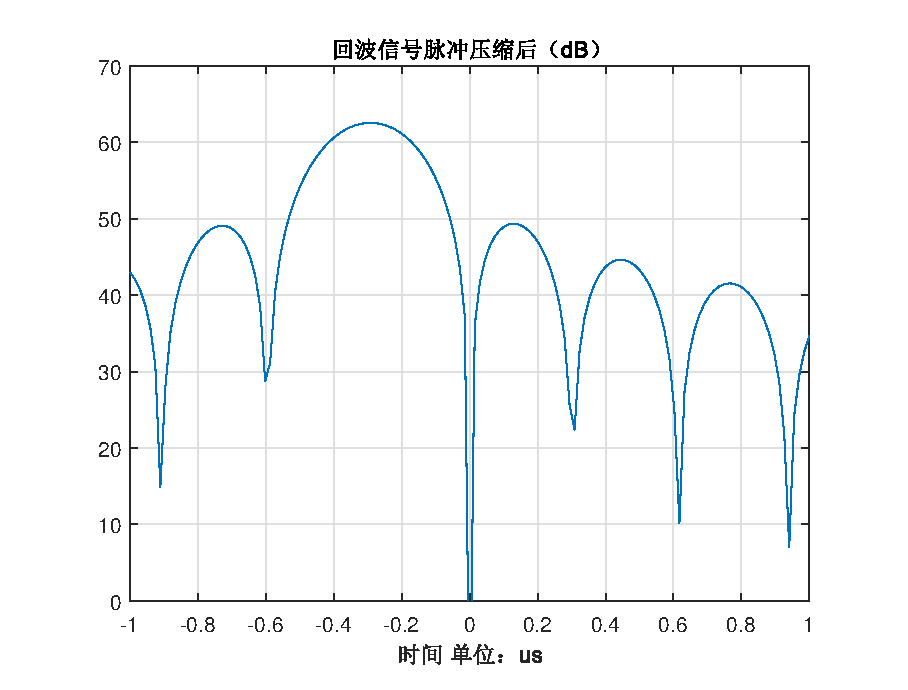
\includegraphics[width=.5\textwidth]{Doppler_sensitivity_0750}\\
    v=700m/s&v=750m/s\\
  \end{tabular}
  \caption{多普勒敏感5}\label{Doppler_sensitivity_0005}
\end{figure}
\begin{figure}[htbp]
  \centering
  \begin{tabular}{cc}
    \includegraphics[width=.5\textwidth]{Doppler_sensitivity_0800}&\includegraphics[width=.5\textwidth]{Doppler_sensitivity_0850}\\
    v=800m/s&v=850m/s\\
    \includegraphics[width=.5\textwidth]{Doppler_sensitivity_0900}&\includegraphics[width=.5\textwidth]{Doppler_sensitivity_0950}\\
    v=900m/s&v=950m/s\\
  \multicolumn{2}{c}{\includegraphics[width=.5\textwidth]{Doppler_sensitivity_1000}}\\
   \multicolumn{2}{c}{v=1000m/s}\\
  \end{tabular}
  \caption{多普勒敏感6}\label{Doppler_sensitivity_0006}
\end{figure}
\begin{figure}[htbp]
  \centering
  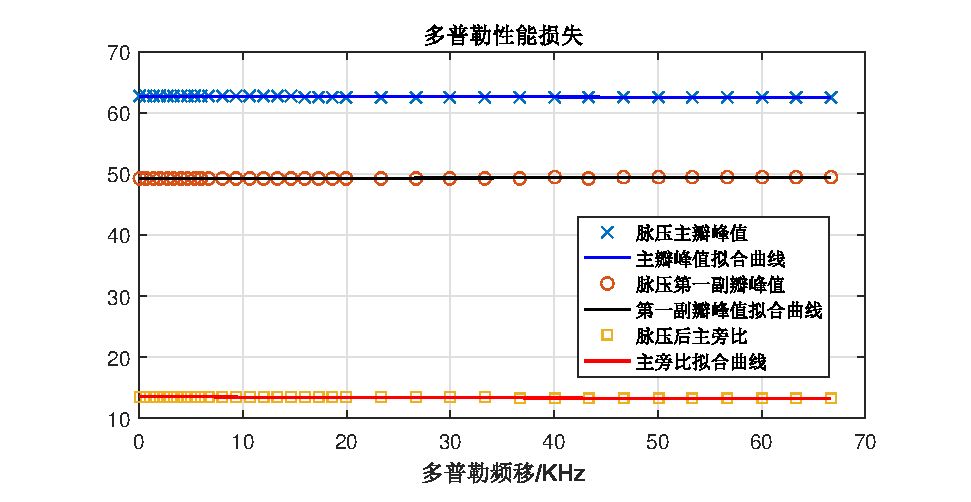
\includegraphics[width=\textwidth]{Doppler_tolerance}
  \caption{多普勒性能损失}\label{Doppler_tolerance}
\end{figure}
\subsection{FFT相干积累}
\subsubsection{FFT表达式及图像}
FFT后的信号表达式为
\begin{equation}\label{FFThou}
  S_{FFT}(\omega)=\int_{-\infty}^{+\infty}s_h(t)e^{j\omega t}\mbox{d}t
\end{equation}\par
在FFT之前,需要进行数据重排,FFT前后的信号图像见图\ref{FFTqianhou}
。\par
\begin{figure}[htbp]
  \centering
  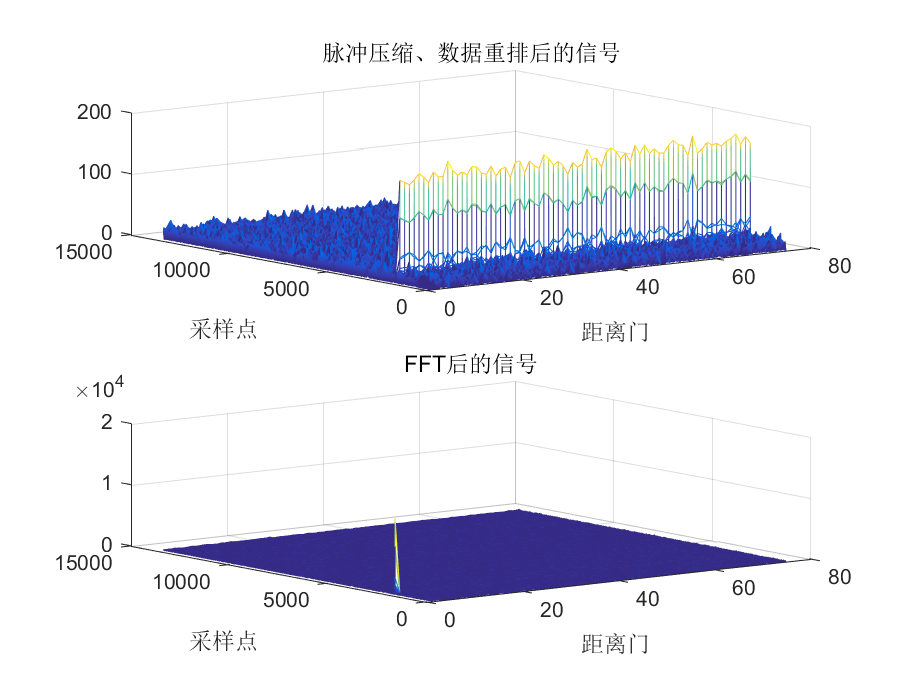
\includegraphics[width=\textwidth]{FFT2}
  \caption{FFT前后图像}\label{FFTqianhou}
\end{figure}
\subsubsection{FFT输出SNR及误差情况分析}
当设定相干积累时间15ms,即相干积累脉冲个数75个时,FFT的理论增益为
\begin{equation}\label{zengyi2}
  G_{theory}=10\lg(M)=10\lg(75)=18.7506\mbox{dB}
\end{equation}
设定输入信噪比$SNR_i=-5$dB,则FFT后的理论输出信噪比${SNR_o}_{thero}=G_{theory}+D_{theory}+SNR_i=42.0757$dB,由图\ref{shuju_FFT}
可知,其实际输出信噪比$SNR_o=42.0473$,相对误差为$0.0675\%$。产生误差的原因可能是匹配滤波本身存在的误差带来的影响。
\begin{figure}[htbp]
  \centering
  \includegraphics[width=.6\textwidth]{TIM20190623132411}
  \caption{FFT输出信噪比}\label{shuju_FFT}
\end{figure}
\subsection{距离模糊和速度模糊}
\subsubsection{距离模糊}
系统的最大单周期测量距离为
\begin{equation}\label{gujizuidazhi}
  R_{max}=\frac{CT}{2}=30000m
\end{equation}
当距离大于30000m后,将无法辨别是第几个周期的回波,产生距离模糊。如图\ref{julimohu1}
及图\ref{julimohu2}
所示,雷达可测得的距离仅为单周期内的距离。
\begin{figure}[htbp]
  \centering
  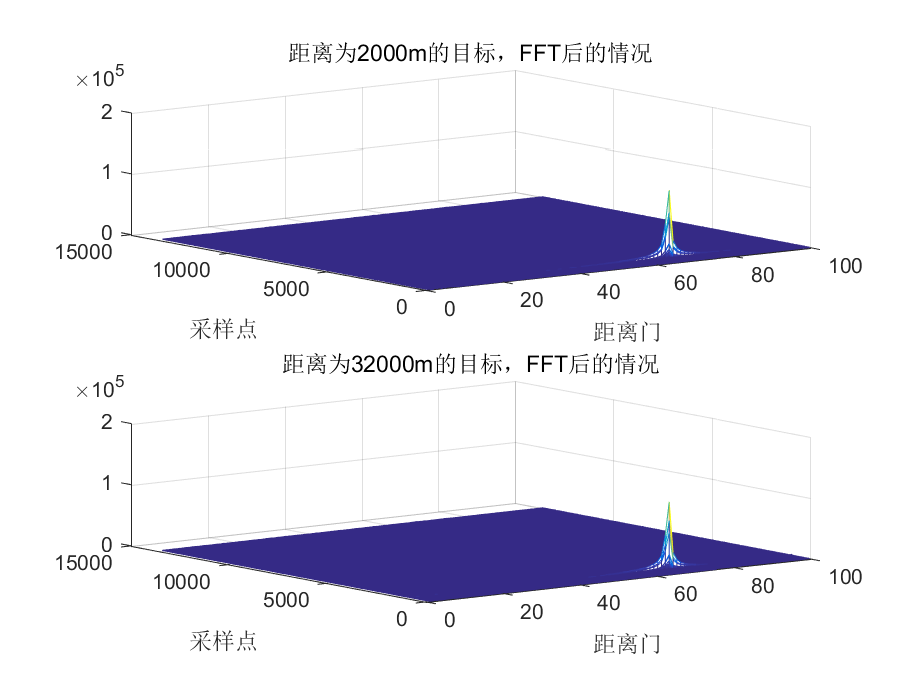
\includegraphics[width=\textwidth]{julimohu1}
  \caption{距离模糊图像}\label{julimohu1}
\end{figure}
\begin{figure}[htbp]
  \centering
  \includegraphics[width=.6\textwidth]{TIM20190623172648}
  \caption{距离模糊时测得的距离}\label{julimohu2}
\end{figure}
\subsubsection{速度模糊}
MTD雷达的多普勒单值测量区间为第一个完整多普勒周期,即$\left[-\frac{f_r}{2},\frac{f_r}{2}\right]$,$f_r$为脉冲重复频率。\par当多普勒频移$f_d$绝对值大于$\frac{f_r}{2}$,将因周期混叠使视在多普勒频移与实际值不符。\par 使得速度不模糊的最大多普勒频移$f_d=\frac{f_r}{2}$,于是最大不模糊速度为
\begin{equation}\label{bumohusudu}
  v=\frac{f_d\lambda}{2}=\frac{f_r\lambda}{4}=37.5m/s
\end{equation}
即速度测量范围为$-37.5m/s\leq v\leq 37.5m/s$。如图\ref{sudumohu1}
及图\ref{sudumohu2}
所示,超过这个范围的速度将产生混叠无法测出。
\begin{figure}[htbp]
  \centering
  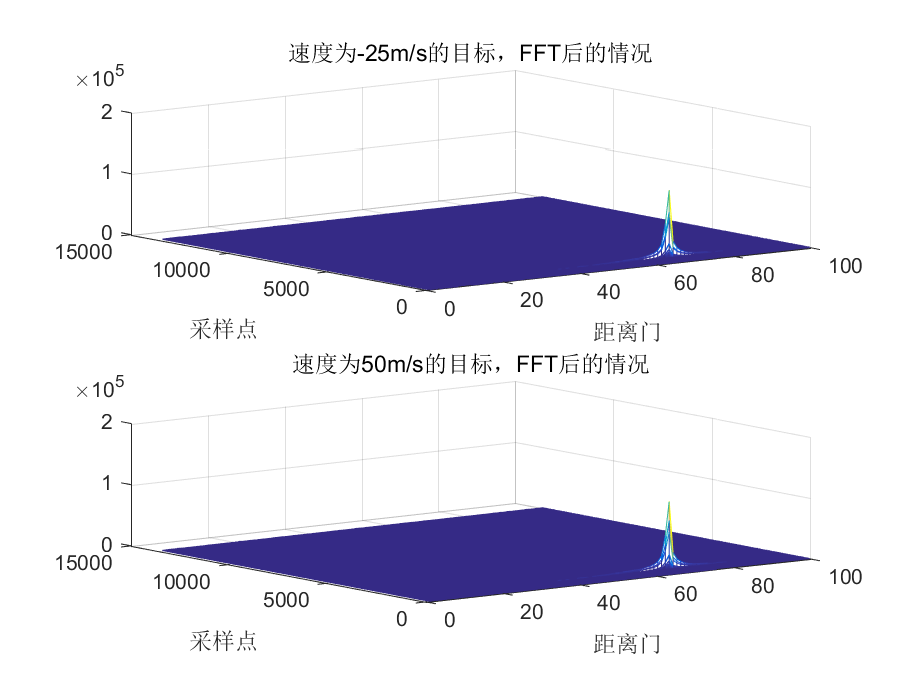
\includegraphics[width=\textwidth]{sudumohu1}
  \caption{速度模糊图像}\label{sudumohu1}
\end{figure}
\begin{figure}[htbp]
  \centering
  \includegraphics[width=.6\textwidth]{TIM20190623225505}
  \caption{速度模糊时测得的距离}\label{sudumohu2}
\end{figure}
\par需要注意的是,在图\ref{sudumohu2}中,由于没有相应的换算(负多普勒频移无法直接体现),事实上是$v_2$的测量值错误了。
\section{双目标时的仿真情况}
\setcounter{table}{0}
\setcounter{figure}{0}
\setcounter{equation}{0}
\subsection{大目标旁瓣掩盖小目标}
\subsubsection{大目标距离旁瓣掩盖小目标}
当两个目标幅度不同,速度相同且距离差值接近且比较巧合时,可能产生距离掩盖小目标的情况,如图\ref{zhegai1}
所示。此时,两目标的幅度分别为8与1。
\begin{figure}[htbp]
  \centering
  \includegraphics[width=\textwidth]{zhegai2}
  \caption{大目标距离旁瓣遮住小目标}\label{zhegai1}
\end{figure}\par
而当两目标的幅度相同时,可以分辨出2个目标,如图\ref{zhegai2}
所示。
\begin{figure}[htbp]
  \centering
  \includegraphics[width=\textwidth]{zhegai1}
  \caption{大小目标幅度大致相等时}\label{zhegai2}
\end{figure}\par
而当两目标的距离差距较大,也可以分辨出2个目标,如图\ref{zhegai3}
所示。
\begin{figure}[htbp]
  \centering
  \includegraphics[width=\textwidth]{zhegai3}
  \caption{大小目标距离、速度相差较大时}\label{zhegai3}
\end{figure}
\subsubsection{大目标速度旁瓣掩盖小目标}
当两个目标幅度不同,距离相同且速度差值接近且比较巧合时,可能产生距离掩盖小目标的情况,如图\ref{zhegai4}
所示。此时,两目标的幅度分别为8与1。
\begin{figure}[htbp]
  \centering
  \includegraphics[width=\textwidth]{zhegai4}
  \caption{大目标速度旁瓣遮住小目标}\label{zhegai4}
\end{figure}
\subsection{距离分辨率与速度分辨率}
\subsubsection{距离分辨}
理论距离分辨率为
\begin{equation}\label{julifenbianlv}
  \Delta r=\frac{C}{2B}=4.41178m
\end{equation}
如图\ref{julifenbianlv1}
所示,当距离差为4m时,无法分辨两个目标。
\begin{figure}[htbp]
  \centering
  \includegraphics[width=\textwidth]{julifenbianlv1}
  \caption{距离上无法分辨}\label{julifenbianlv1}
\end{figure}\par
而当距离差为6m时,如图\ref{julifenbianlv2}
所示,可以分辨出两个目标。
\begin{figure}[htbp]
  \centering
  \includegraphics[width=\textwidth]{julifenbianlv2}
  \caption{距离上可以分辨}\label{julifenbianlv2}
\end{figure}
\subsubsection{速度分辨}
理论上区分两个运动目标的最小多普勒频移为
\begin{equation}\label{julifenbianlv21}
  \Delta f_d=\frac{1}{T_a}
\end{equation}
即为相干积累时间的倒数,为了让速度分辨更明显,设置相干积累时间为10ms。则对应的速度分辨率为
\begin{equation}\label{sudufenblv2}
  \Delta v=\frac{\Delta f_d\lambda}{2}=1.5m/s
\end{equation}
如图\ref{sudufenbianlv1}
所示,仿真中,当速度差为1m/s时,无法分辨两目标。
\begin{figure}[htbp]
  \centering
  \includegraphics[width=\textwidth]{sudufenbianlv1}
  \caption{速度上无法分辨}\label{sudufenbianlv1}
\end{figure}\par
而当速度差为3m/s时,如图\ref{sudufenbianlv2}
所示,可以分辨出两个目标。
\begin{figure}[htbp]
  \centering
  \includegraphics[width=\textwidth]{sudufenbianlv2}
  \caption{速度上可以分辨}\label{sudufenbianlv2}
\end{figure}
\newpage
\section{MATLAB程序代码}
\subsection{发射信号与自相关函数}
\zihao{5}
\begin{lstlisting}
clc;
clear;
B=34e6;                 %带宽
T=200e-6;                 %周期
D=10e-2;            %占空比
Fc=10e9;            %载频
SNRi=-25;              %输入信噪比
V=0;              %目标速度
A=3;               %目标幅度
R=0;            %目标距离
tt=10e-3;           %相干积累时间
%******************常数或中间参数*******************
Tau=D*T;                %脉宽
K=B/Tau;              %线性调频斜率
Fs=2*B;             %采样频率
Ts=1/Fs;            %采样周期
C=3e8;              %光速C
M=tt/T;             %脉冲重复个数
%******************线性调频信号***************
N=round(T/Ts);
t1=linspace(-Tau/2,Tau/2,N*D);
t=linspace(-T/2,T/2,N);
St_0=exp(2*j*pi*(+0.5*K*t1.^2));
N1=round(N*(1-D)/2);
zero=zeros(1,N1);%补零
St=[zero,St_0,zero];
%LFM时域波形
 figure(1);
 subplot(2,1,1)
 plot(t*1e6,real(St));
 xlabel('时间 单位:us');
 title('线性调频信号时域波形');
 grid on;axis tight;
%LFM频域波形
 f=linspace(-Fs/2,Fs/2,N);
 figure(1);
 subplot(2,1,2)
 fftshift(abs(fft(St)));
 St_FFT=fftshift(abs(fft(St)));
 plot(f*1e-6,St_FFT);
 xlabel('频率 单位:MHz');
 title('线性调频信号幅频特性');
 grid on;axis tight;
%***************自相关函数*********************
Ht_0=fliplr(St);
Ht=conj(Ht_0);
Sot=conv(St,Ht);
N2=2*N-1;
t2=linspace(-T,T,N2);
Z0=abs(Sot);
%自相关函数
 figure(2)
 subplot(2,1,1)
 plot(t2*1e6,Z0);
 axis([-21,21,-inf,inf]);grid on;
 xlabel('时间 单位:us');
 title('自相关函数');
%自相关函数dB
 figure(2)
 subplot(2,1,2)
Z1=20*log10(Z0);
 plot(t2*1e6,Z1);
 axis([-21,21,-inf,inf]);grid on;
 xlabel('时间 单位:us');
 title('自相关函数(dB)');
%自相关函数放大
 figure(3)
 subplot(2,1,1)
 plot(t2*1e6,Z1);
 axis([-0.1,0.1,-5,70]);grid on;
 xlabel('时间 单位:us');
 title('自相关函数(dB)');
%自相关函数放大2
 figure(3)
 subplot(2,1,2)
Z0=Z0/max(Z0);
Z2=20*log10(Z0);
 plot(t2*1e6,Z2);
 axis([-0.1,0.1,-5,1]);grid on;
 xlabel('时间 单位:us');
 title('自相关函数(归一化)');
%查找自相关函数参数

 t_find=linspace(-0.6e-6,0.6e-6,N*100);%插值范围
 Z_1=interp1(t2,Z1,t_find,'linear'); %内插值
 Z_2=interp1(t2,Z2,t_find,'linear'); %内插值
 range=double(-0.2*1e-6);[para1,para2] = find(t_find<=range);
 m_1_1=max(para2);
 range=double(0.2*1e-6);[para1,para2] = find(t_find<=range);
 m_1_2=max(para2);
 max_Main_Lobe=max(Z_1(:));%主瓣高度
 range=double(0.03*1e-6);[para1,para2] = find(t_find<=range);
 m_1_1=max(para2);
 range=double(0.06*1e-6);[para1,para2] = find(t_find<=range);
 m_1_2=max(para2);
 max_Side_Lobe=max(Z_1(m_1_1:m_1_2));%第一旁瓣
 Main_lobe_side_lobe_ratio=max_Main_Lobe-max_Side_Lobe;%主瓣旁瓣比
 range=double(-4);[para1,para2] = find(Z_2>=range);
 m_1_1=max(para2);
 m_1_2=min(para2);
 max_4dB_Output_Pulse_Width=(t_find(m_1_1)-t_find(m_1_2))*1e9;%4dB输出带宽
\end{lstlisting}
\subsection{匹配滤波与脉压输出信噪比}
\begin{lstlisting}
clc;
clear;
B=34e6;                 %带宽
T=200e-6;                 %周期
D=10e-2;            %占空比
Fc=10e9;            %载频
SNRi=-5;              %输入信噪比
V=0;              %目标速度
A=1;               %目标幅度
R=4000;            %目标距离
tt=15e-3;           %相干积累时间
%******************常数或中间参数*******************
Tau=D*T;                %脉宽
K=B/Tau;              %线性调频斜率
fs=2*B;             %采样频率
Ts=1/fs;            %采样周期
C=3e8;              %光速C
M=tt/T;             %脉冲重复个数
%******************线性调频信号***************
N=round(T/Ts);
t1=linspace(-Tau/2,Tau/2,N*D);
t_0=linspace(-T/2,T/2,N);
St_0=exp(j*pi*K*t1.^2);
N1=round(N*(1-D)/2);
f=linspace(-fs/2,fs/2,N);
zero=zeros(1,N1);%补零
St=[St_0,zero,zero];
St_repeat=repmat(St,1,M);
%***************回波信号**********************
fd=2*V/(C/Fc);%多普勒频移
i=1:N*M;
St_Dop=exp(2*j*pi*fd*Ts*i);%多普勒延时频移信号部分
i=1:N;
St_Dop1=exp(2*j*pi*fd*Ts*i);
t_Delay=2*R/C;  %延时
N_R=round(t_Delay/Ts);
zero_left=zeros(1,N_R);
zero_right=zeros(1,2*N1-N_R);
St1=A*[zero_left,St_0,zero_right];
St_00=A*[zero_left,St_repeat];
i=1:M*N;
St_1(i)=St_00(i);
St_M=St_1.*St_Dop;%带多普勒频移的信号
t_1=linspace(-Tau/2,T-Tau/2,N);
St_=St.*St_Dop1;
figure(1)
subplot(211);
plot(t_1*1E6,real(St_));
xlabel('时间 单位:us');
 title('LFM信号');
 grid on;axis tight;
subplot(212);
plot(t_1*1E6,real(St1));
xlabel('时间 单位:us');
 title(['延时为',num2str(t_Delay*1e6),'\mus的回波信号']);
 grid on;axis tight;
St_M_Gauss=randn(1,size(St_M,2))+j*randn(1,size(St_M,2));%产生白噪声
 [filterB,filterA] = butter(12,0.5,'low');%20阶低通巴特沃斯滤波器
 [h,w]=freqz(filterB,filterA);
 St_M_Gauss=filter(filterB,filterA,St_M_Gauss);
P_Ni=sum(abs(St_M_Gauss).^2)/length(St_M_Gauss);
P_Si= P_Ni.*(10.^(SNRi/10));
St_M_without=sqrt(P_Si)*St_M;
St_M_with=St_M_without+St_M_Gauss;
figure(11);
subplot(211);
plot(fftshift(abs(fft(St_M_Gauss))).^2);
title('滤波后的白噪声功率谱');
subplot(212);
plot(fftshift(abs(fft(St_M))).^2);
title('信号功率谱');
%*************匹配滤波(脉冲压缩)************
Ht_0=fliplr(St);
Ht=conj(Ht_0);
St_H_without=conv(St_M_without,Ht);
St_H_Gauss=conv(St_M_Gauss,Ht);
St_H_with=conv(St_M_with,Ht);
P_So=max(abs(St_H_without).^2);
P_So_dB=10*log10(P_So);
P_No=sum(abs(St_H_Gauss).^2)/length(St_H_Gauss);
P_No_dB=10*log10(P_No);
D_thero=10*log10(B*Tau);
SNRo_thero=D_thero+SNRi;
SNRo=P_So_dB-P_No_dB;
N2=N*M;
t_2=linspace(0,T*(M+1),N2);
N3=N*(M+1)-1;
t_3=linspace(0,T*(M+1),N3);
figure(2)
subplot(211);
plot(t_2*1E6,real(St_M_with));
xlabel('时间 单位:us');
 title('加入噪声的回波信号');
 grid on;axis tight;
subplot(212);
plot(t_3*1E6,real(St_H_with));
xlabel('时间 单位:us');
 title('脉冲压缩后的信号');
 grid on;axis tight;
\end{lstlisting}
\subsection{多普勒敏感与多普勒容限}
\begin{lstlisting}
clc;
clear;
B=34e6;                 %带宽
T=200e-6;                 %周期
D=10e-2;            %占空比
Fc=10e9;            %载频
SNRi=-25;              %输入信噪比
V=1000;              %目标速度
A=1;               %目标幅度
R=0;            %目标距离
tt=10e-3;           %相干积累时间
%******************常数或中间参数*******************
Tau=D*T;                %脉宽
K=B/Tau;              %线性调频斜率
Fs=2*B;             %采样频率
Ts=1/Fs;            %采样周期
C=3e8;              %光速C
M=tt/T;             %脉冲重复个数
%******************线性调频信号***************
N=round(T/Ts);
t1=linspace(-Tau/2,Tau/2,N*D);
t=linspace(-T/2,T/2,N);
St_0=exp(j*pi*K*t1.^2);
N1=round(N*(1-D)/2);
zero=zeros(1,N1);%补零
St=[zero,St_0,zero];
%*******************回波信号**************
fd=2*V/(C/Fc);%多普勒频移
St_Dop=exp(2*j*pi*fd.*t);%多普勒延时频移信号部分
t_Delay=mod(2*R/C,T);
N_R=round(t_Delay/Ts);
zero_left=zeros(1,N1+N_R);
zero_right=zeros(1,N1-N_R);
St1=A*[zero_left,St_0,zero_right];
St_M=St1.*St_Dop;
%****************脉冲压缩(匹配滤波)************
Ht_0=fliplr(St);
Ht=conj(Ht_0);
Sot=conv(St_M,Ht);
N2=2*N-1;
t2=linspace(-T,T,N2);
Z0=abs(Sot);
Z1=20*log10(Z0);
%脉冲压缩图像放大
 figure(3)
 plot(t2*1e6,Z1);
 axis([-1,1,0,70]);grid on;
 xlabel('时间 单位:us');
 title('回波信号脉冲压缩后(dB)');
Z0=Z0/max(Z0);
Z2=20*log10(Z0);
%查找相关参数
range=double(-2*1e-6);[para1,para2] = find(t2<=range);
m_1_1=max(para2);
range=double(2*1e-6);[para1,para2] = find(t2<=range);
m_1_2=max(para2);
max_Main_Lobe=max(Z1(m_1_1:m_1_2));%主瓣高度
range=double(0.3*1e-6);[para1,para2] = find(t2<=range);
m_1_1=max(para2);
range=double(0.6*1e-6);[para1,para2] = find(t2<=range);
m_1_2=max(para2);
max_Side_Lobe_para1=max(Z1(m_1_1:m_1_2));
range=double(-0.6*1e-6);[para1,para2] = find(t2<=range);
m_1_1=max(para2);
range=double(-0.3*1e-6);[para1,para2] = find(t2<=range);
m_1_2=max(para2);
max_Side_Lobe_para2=max(Z1(m_1_1:m_1_2));
max_Side_Lobe=max([max_Side_Lobe_para1,max_Side_Lobe_para2]);%第一旁瓣
range=double(-4);[para1,para2] = find(Z2>=range);
m_1_1=max(para2);
m_1_2=min(para2);
max_4dB_Output_Pulse_Width=(t2(m_1_1)-t2(m_1_2))*1e9;%4dB输出带宽
Main_lobe_side_lobe_ratio=max_Main_Lobe-max_Side_Lobe;%脉压主旁比
\end{lstlisting}
\subsection{FFT}
\begin{lstlisting}
clc;
clear;
B=34e6;                 %带宽
T=200e-6;                 %周期
D=10e-2;            %占空比
Fc=10e9;            %载频
SNRi=-5;              %输入信噪比
V=0;              %目标速度
A=1;               %目标幅度
R=4000;            %目标距离
tt=15e-3;           %相干积累时间
%******************常数或中间参数*******************
Tau=D*T;                %脉宽
K=B/Tau;              %线性调频斜率
fs=2*B;             %采样频率
Ts=1/fs;            %采样周期
C=3e8;              %光速C
M=tt/T;             %脉冲重复个数
%******************线性调频信号***************
N=round(T/Ts);
t1=linspace(-Tau/2,Tau/2,N*D);
t_0=linspace(-T/2,T/2,N);
St_0=exp(j*pi*K*t1.^2);
N1=round(N*(1-D)/2);
f=linspace(-fs/2,fs/2,N);
zero=zeros(1,N1);%补零
St=[zero,St_0,zero];
%***************回波信号**********************
fd=2*V/(C/Fc);%多普勒频移
i=1:N*(M+1);
St_Dop=exp(2*j*pi*fd*Ts*i);%多普勒延时频移信号部分
t_Delay=2*R/C;  %延时
N_R=round(t_Delay/Ts);
zero_left=zeros(1,N1+N_R);
St_repeat=repmat(St,1,(M+1));
St_1=A*[zero_left,St_repeat];
St_1=St_1(:,1:(M+1)*N);
St_M=St_1.*St_Dop;%带多普勒频移的信号
t_1=linspace(0,T,N);
St_M_Gauss=randn(1,size(St_M,2))+j*randn(1,size(St_M,2));%产生白噪声
 [filterB,filterA] = butter(12,0.5,'low');%20阶低通巴特沃斯滤波器
 [h,w]=freqz(filterB,filterA);
 St_M_Gauss=filter(filterB,filterA,St_M_Gauss);

 P_Ni=sum(abs(St_M_Gauss).^2)/length(St_M_Gauss);
P_Si= P_Ni.*(10.^(SNRi/10));
St_M_without=sqrt(P_Si)*St_M;
St_M_with=St_M_without+St_M_Gauss;
%*************匹配滤波(脉冲压缩)************
Ht_0=fliplr(St);
Ht=conj(Ht_0);
St_H_without=conv(St_M_without,Ht);
St_H_Gauss=conv(St_M_Gauss,Ht);
St_H_with=conv(St_M_with,Ht);
A_thero=10*log10(B*Tau)+10*log10(M);
SNRo_thero=A_thero+SNRi;
%*********************数据重排***********
 for r=1:M
for h=1:N
position=(r-1)*N+h+N*(1-D)/2;
St_fft_arrange_without(h,r)=St_H_without(position);
St_fft_arrange_Gauss(h,r)=St_H_Gauss(position);
St_fft_arrange_with(h,r)=St_H_with(position);
end
 end
figure(5);
subplot(211);
mesh(1:M,1:N,abs(real(St_fft_arrange_with)));
xlabel('距离门');
ylabel('采样点');
title('脉冲压缩、数据重排后的信号');
%*******************FFT*********************
for h=1:N
St_fft_without(h,:)=abs(fft(St_fft_arrange_without(h,:)));
St_fft_Gauss(h,:)=abs(fft(St_fft_arrange_Gauss(h,:)));
St_fft_with(h,:)=abs(fft(St_fft_arrange_with(h,:)));
end
figure(5);
subplot(212);
mesh(1:M,1:N,(St_fft_with));
xlabel('距离门');
ylabel('采样点');
title('FFT后的信号');
A_So=max(max(St_fft_without));
P_So=A_So^2;
P_So_dB=10*log10(P_So);
P_No=sum(sum(abs(St_fft_Gauss.^2)))/(N*M);
P_No_dB=10*log10(P_No);
SNRo=P_So_dB-P_No_dB;
\end{lstlisting}
\subsection{距离模糊与速度模糊}
\begin{lstlisting}
clc;
clear;
B=34e6;                 %带宽
T=200e-6;               %周期
D=10e-2;            %占空比
Fc=10e9;            %载频
SNRi=-5;              %输入信噪比
V1=-25;              %目标速度1
V2=50;           %速度2
A=1;               %目标幅度
R1=2000;            %距离1
R2=32000;          %距离2
tt=20e-3;           %相干积累时间
%******************常数或中间参数*******************
Tau=D*T;                %脉宽
K=B/Tau;              %线性调频斜率
fs=2*B;             %采样频率
Ts=1/fs;            %采样周期
C=3e8;              %光速C
M=tt/T;             %脉冲重复个数
%******************线性调频信号***************
N=round(T/Ts);
t1=linspace(-Tau/2,Tau/2,N*D);
t_0=linspace(-T/2,T/2,N);
St_0=exp(j*pi*K*t1.^2);
N1=round(N*(1-D)/2);
f=linspace(-fs/2,fs/2,N);
zero=zeros(1,N1);%补零
St=[zero,St_0,zero];
%***************回波信号**********************
St_repeat=repmat(St,1,M+1);
t_Delay1=2*R1/C;     t_Delay2=2*R2/C; %延时
N_R1=round(t_Delay1/Ts);N_R2=round(t_Delay2/Ts);
zero_left1=zeros(1,N1+N_R1);zero_left2=zeros(1,N1+N_R2);
St1=A*[zero_left1,St_repeat];       St2=A*[zero_left2,St_repeat];
St1=St1(:,1:(M+1)*N);    St2=St2(:,1:(M+1)*N);
fd1=2*V1/(C/Fc);     fd2=2*V2/(C/Fc);%多普勒频移
i=1:N*(M+1);
St_Dop1=exp(2*j*pi*fd1*Ts*i);       St_Dop2=exp(2*j*pi*fd2*Ts*i);%多普勒延时频移信号部分
St_M1=St1.*St_Dop1;     St_M2=St2.*St_Dop2;%带多普勒频移的信号
St_M_Gauss=randn(1,size(St_M1,2))+j*randn(1,size(St_M1,2));%产生白噪声
 [filterB,filterA] = butter(12,0.5,'low');%20阶低通巴特沃斯滤波器
 [h,w]=freqz(filterB,filterA);
 St_M_Gauss=filter(filterB,filterA,St_M_Gauss);
St_M_with1=St_M1+St_M_Gauss;    St_M_with2=St_M2+St_M_Gauss;
%*************匹配滤波(脉冲压缩)************
Ht_0=fliplr(St);
Ht=conj(Ht_0);
St_H_with1=conv(St_M_with1,Ht);     St_H_with2=conv(St_M_with2,Ht);
%*********************数据重排***********
 for r=1:M
for h=1:N
position=(r-1)*N+h+N*(1-D)/2;
St_fft_arrange_with1(h,r)=St_H_with1(position);
St_fft_arrange_with2(h,r)=St_H_with2(position);
end
 end
%*******************FFT*********************
for h=1:N
St_fft_with1(h,:)=(abs(fft(St_fft_arrange_with1(h,:))));
St_fft_with2(h,:)=(abs(fft(St_fft_arrange_with2(h,:))));
end

figure(5);
subplot(211);
mesh(1:M,1:N,(St_fft_with1));
xlabel('距离门');
ylabel('采样点');
title(['距离为',num2str(R1),'m的目标,FFT后的情况']);
subplot(212);
mesh(1:M,1:N,(St_fft_with2));
xlabel('距离门');
ylabel('采样点');
title(['距离为',num2str(R2),'m的目标,FFT后的情况']);
[para1_1 para1_2]=max(max(St_fft_with1,[],2));
R1_Calculated=para1_2/N*T*C/2;
[para2_1 para2_2]=max(max(St_fft_with2,[],2));
R2_Calculated=para2_2/N*T*C/2;

figure(6);
subplot(211);
mesh(1:M,1:N,(St_fft_with1));
xlabel('距离门');
ylabel('采样点');
title(['速度为',num2str(V1),'m/s的目标,FFT后的情况']);
subplot(212);
mesh(1:M,1:N,(St_fft_with2));
xlabel('距离门');
ylabel('采样点');
title(['速度为',num2str(V2),'m/s的目标,FFT后的情况']);
[para1_1 para1_2]=max(max(St_fft_with1,[],1));
V1_Calculated=para1_2/M*C/T/2/Fc;
[para2_1 para2_2]=max(max(St_fft_with2,[],1));
V2_Calculated=para2_2/M*C/T/2/Fc;
\end{lstlisting}
\subsection{双目标}
\begin{lstlisting}
clc;
clear;
B=34e6;                 %带宽
T=200e-6;               %周期
D=10e-2;            %占空比
Fc=10e9;            %载频
SNRi=-5;              %输入信噪比
V1=20;              %目标速度1
V2=22;           %速度2
A1=8;               %目标幅度
A2=8;            %目标幅度
tt=10e-3;           %相干积累时间
%******************常数或中间参数*******************
Tau=D*T;                %脉宽
K=B/Tau;              %线性调频斜率
fs=2*B;             %采样频率
Ts=1/fs;            %采样周期
C=3e8;              %光速C
M=tt/T;             %脉冲重复个数
%******************线性调频信号***************
R1=60;            %距离1
R2=60;          %距离2

N=round(T/Ts);
t1=linspace(-Tau/2,Tau/2,N*D);
t_0=linspace(-T/2,T/2,N);
St_0=exp(j*pi*K*t1.^2);
N1=round(N*(1-D)/2);
f=linspace(-fs/2,fs/2,N);
zero=zeros(1,N1);%补零
St=[zero,St_0,zero];
%***************回波信号**********************
St_repeat=repmat(St,1,M+1);
t_Delay1=2*R1/C;     t_Delay2=2*R2/C; %延时
N_R1=round(t_Delay1/Ts);N_R2=round(t_Delay2/Ts);
zero_left1=zeros(1,N1+N_R1);zero_left2=zeros(1,N1+N_R2);
St1=A1*[zero_left1,St_repeat];       St2=A2*[zero_left2,St_repeat];
St1=St1(:,1:(M+1)*N);    St2=St2(:,1:(M+1)*N);
fd1=2*V1/(C/Fc);     fd2=2*V2/(C/Fc);%多普勒频移
i=1:N*(M+1);
St_Dop1=exp(2*j*pi*fd1*Ts*i);       St_Dop2=exp(2*j*pi*fd2*Ts*i);%多普勒延时频移信号部分
St_M=St1.*St_Dop1+St2.*St_Dop2;%带多普勒频移的信号
St_M_Gauss=randn(1,size(St_M,2))+j*randn(1,size(St_M,2));%产生白噪声
 [filterB,filterA] = butter(12,0.5,'low');%20阶低通巴特沃斯滤波器
 [h,w]=freqz(filterB,filterA);
 St_M_Gauss=filter(filterB,filterA,St_M_Gauss);
St_M_with=St_M+St_M_Gauss;
%*************匹配滤波(脉冲压缩)************
Ht_0=fliplr(St);
Ht=conj(Ht_0);
St_H_with=conv(St_M_with,Ht);
%*********************数据重排***********
 for r=1:M
for h=1:N
position=(r-1)*N+h+N*(1-D)/2;
St_fft_arrange_with(h,r)=St_H_with(position);
end
 end
%*******************FFT*********************
for h=1:N
St_fft_with(h,:)=(abs(fft(St_fft_arrange_with(h,:))));
end
%*******************数据抽取*****************
k=60;
for h=1:k
    St_fft_with_chose(h,:)=St_fft_with(h,:);
end

%*******************距离分辨率*************
figure(6);
subplot(311);
mesh(1:M,1:k,(St_fft_with_chose));
xlabel('距离门');
ylabel('采样点');
title(['距离差为',num2str(abs(R2-R1)),'m的情况']);
figure(6);
subplot(312);
mesh(1:M,1:k,(St_fft_with_chose));
view(-90,0);
title(['距离投影']);
subplot(313);
mesh(1:M,1:k,(St_fft_with_chose));
view(0,0);
title(['速度投影']);

%*******************速度分辨率*************
figure(7);
subplot(311);
mesh(1:M,1:k,(St_fft_with_chose));
xlabel('距离门');
ylabel('采样点');
title(['速度差为',num2str(abs(V2-V1)),'m/s的情况']);
figure(7);
subplot(312);
mesh(1:M,1:k,(St_fft_with_chose));
view(-90,0);
title(['距离投影']);
figure(7);
subplot(313);
mesh(1:M,1:k,(St_fft_with_chose));
view(0,0);
title(['速度投影']);

%*******************遮盖*************
figure(8);
subplot(311);
mesh(1:M,1:k,(St_fft_with_chose));
xlabel('距离门');
ylabel('采样点');
title(['距离差',num2str(abs(R2-R1)),'m 速度差',num2str(abs(V2-V1)),'m/s']);
figure(8);
subplot(312);
mesh(1:M,1:k,(St_fft_with_chose));
view(-90,0);
title(['距离投影']);
figure(8);
subplot(313);
mesh(1:M,1:k,(St_fft_with_chose));
view(0,0);
title(['速度投影']);
\end{lstlisting}
\end{document}
